% !TEX program = xelatex

\usepackage{tikz}

\counterwithout{figure}{section}
\counterwithout{table}{section}
\counterwithout{equation}{section}

\titleformat{\subsection}[block]
  {\bfseries\filcenter}{#1}{0cm}{}
\titlespacing{\subsection}{0cm}{21pt}{21pt}

\DeclareCaptionLabelFormat{gosttable}{Таблица #2}

\usepackage{float}
\usepackage{pgfplots}
\usepackage{graphicx}
\usepackage{multirow}
\usepackage{amssymb,amsfonts,amsmath,amsthm}

\usepackage{listings}
\lstset{basicstyle=\footnotesize\ttfamily,breaklines=true}
\lstset{language=Matlab}

\lstdefinelanguage{Python}{
  keywords={and, break, class, continue, def, yield, del, elif, else, except, exec, finally, for, from, global, if, import, in, lambda, not, or, pass, print, raise, return, try, while, assert, with},
  keywordstyle=\color{NavyBlue}\bfseries,
  ndkeywords={True, False},
  ndkeywordstyle=\color{BurntOrange}\bfseries,
  emph={as},
  emphstyle={\color{OrangeRed}},
  identifierstyle=\color{black},
  sensitive=true,
  commentstyle=\color{gray}\ttfamily,
  comment=[l]{\#},
  morecomment=[s]{/*}{*/},
  stringstyle=\color{ForestGreen}\ttfamily,
  morestring=[b]',
  morestring=[s]{"""*}{*"""},
}


\usepackage{lastpage}
\usepackage{calc}
\usepackage{soul}
\usepackage{pbox}
\usepackage{ulem}
\usepackage{titling}
\usepackage{framed}
\usepackage{tabu}
\usepackage{lscape}
\usepackage{appendix}
\usepackage{pdflscape}
\usepackage{longtable}
\usepackage[figure,table]{totalcount}

\graphicspath{{figures/}}
\addbibresource{bibliography.bib}

\begin{document}
\Ukrainian

\addtocounter{page}{1}
\renewcommand\contentsname{\hspace*{\fill}\bfseries\MakeUppercase{Зміст}\hspace*{\fill}}
\tableofcontents


\section*{Вступ}
\addcontentsline{toc}{section}{Вступ}
Через стрімкий перехід на онлайн джерела новин, медіа простір переживає різкі зміни.
На відміну від традиційних офлайн джерел новин, де лояльність її читачів статична через недостатній об'єм вибору, для онлайн джерел існує величезний вибір: від локальних видавництв до міжнародних та нішевих.
Це змушує онлайн джерела використовувати всі можливі способи заманити читача на свою сторінку новин --- клікбейт.

Клекбейт заснований на феномені пізнання, який базується на інтересі людини до вивчення нових знань. Клекбейт заголовки породжують цікавість але задовольняють його, змушуючи читача перейти на сторінку новини.
В результаті текст статті викликає тільки розчарування, так як він не може задовольнити цікавість викликану заголовком.

Об'єктом роботи є процес класифікації новинних статей за рівнем "клікбейтності".

Предметом роботи є моделі та інструментальні засоби для розробки системи КНС за рівнем "клікбейтності".

Актуальністю роботи є наростаюча популярність новинних статей, метою яких в першу чергу є залучення аудиторії, а не подача якісної і точної інформації.

Метою роботи є розробка та дослідження моделей і програмна реалізація прототипу системи для КНС за рівнем "клікбейтності".

\section{Підходи до автоматичної оцінки <<клікбейтності>> текстів}
Оцінка клікбейтності заголовків є відносно новою областю. 

В недавніх работах з цієї теми використовуються \textit{self-attentive} нейронні мережі для автоматичного анализу потоку заголовків~\cite{Chopra2017}. 
Альтернативним популярним методом є використання груп лінійних SVM моделей~\cite{Joulin2016}.

Існують різні подходи для классификації невеликих текстів~\cite{Joulin2016}:
\begin{enumerate}
    \item Підходи, засновані на правилах. Переваги: ​​найбільш точний. Недоліки: дуже сильно залежить від предметної області; вимагає великих ресурсів для розробки.
    \item Підходи, засновані на словниках. Переваги: ​​простий у застосуванні. Недоліки: не точний; залежить від предметної області.
    \item Підходи, засновані на машинному навчанні з учителем. Переваги: ​​автоматичний; точний. Недоліки: вимагає великої кількості даних і ресурсів для навчання.
    \item Підходи, засновані на машинному навчанні без учителя. Переваги: ​​автоматичний; не вимагає дані для навчання. Недоліки: не точний.
\end{enumerate}

\section{Модель системи}
Як основу моделі нейронної мережі було обрано LSTM нейронна мережа. 
LSTM мережі являють собою підтип рекурентних нейронних мереж, здатних до вивчення довгих ланцюгов залежностей~\cite{Hochreiter1997}. 
Архітектура такої моделі дозволяє накопичувати інформацію на протязі виконання та використовує звороній зв'язок щоб запам'ятати минулий стан нейронів~\cite{Christopher2015}.

Архитектура мережі представлена на рисунку~\ref{fig:approach_model}.

\begin{figure}[H]
    \centering
    \includegraphics[width=0.25\textwidth]{approach_model}
    \caption{Запропонована модель}
    \label{fig:approach_model}
\end{figure}

Нехай заголовок статті має $N$ токенів, тоді перетворимо кожен токен $w_n$, де $n \in [1, N]$ до векторного представлення $x_n$ за використанням матриці векторного представлення слів $W_E \in \mathbb{R}^{V \times d_0}$, де $d_0$ визначає вимір вектору, а $V$ --- розмір словаря. 

Використаємо однонаправлену LSTM для кодування контекстної информації:
\[
    \vec{h_n} = LSTM(x_n, \vec{h_{n-1}}),
\]
де $\vec{h_n} \in \mathbb{R}^{d_1}$.

Вектор важливості $\alpha \in \mathbb{R}^N$:
\[
    \alpha = softmax(\tanh(H W_H) \cdot v),
\]
де $H = \{ h_1, h_2, \dots, h_N \}$ та $H \in \mathbb{R}^{N \times 2d_1}$.

Векторне представлення заголовку статті:
\[
    s = H^T \alpha,
\]
де $s \in \mathbb{R}^{2d_1}$.

Прогноз принадлежності заголовку до категорій $p = { p_1, p_2 }$:
\[
    p = softmax(W_s s + b_s),
\]
де $W_s \in \mathbb{R}^{4\times 2d_1}$ та $b_s \in \mathbb{R}$ --- параметри які потрібно корегувати при тренуванні.

\section{Проектування системи}
\subsection{Розробка вимог до програмної системи}
\subsubsection{Галузь застосування}
Данний продукт може бути використаний як додаток до броузеру читача, або у пошукових системах.

\subsubsection{Функціональні вимоги}
Функціональних вимоги до системи представлені у виді діаграми прецедентів на рисунку~\ref{fig:use_case}:

\begin{figure}[H]
	\centering
	\includegraphics[width=\textwidth]{use_case}
	\caption{UML-діаграма прецедентів}
	\label{fig:use_case}
\end{figure} 

\subsubsection{Нефункціональні вимоги}
Список нефункціональних вимог до системи:
\begin{enumerate}[label={\arabic*)}]
	\item файли для завантаження повинні мати JSON формат;
    \item виклики зовнішнього API мають бути можливі з консолі;
    \item система повинна мати точність вище або рівну 75\%;
    \item система повинна підтримувати класифікацію статей тільки англійською мовою.
\end{enumerate}

Список атрибутів якості системи:
\begin{enumerate}[label={\arabic*)}]
	\item переносимість;
    \item ефективність;
    \item сопровождаемость.
\end{enumerate}

\subsubsection{Діаграма класів}
Діаграмма классів системи представлена на рисунку~\ref{fig:class}:

\begin{figure}[H]
	\centering
	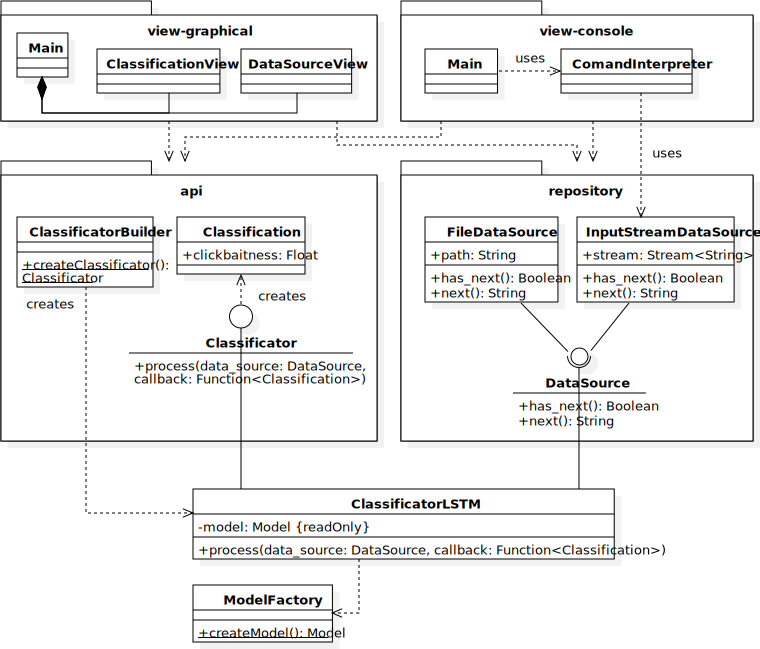
\includegraphics[width=\textwidth]{class}
	\caption{UML-діаграма класів}
	\label{fig:class}
\end{figure} 

\section{Тренування та перевірка моделі}
\subsection{Тренування моделі}
LSTM нейронна мережа пройшла тренування з використанням функції втрат <<перехресна ентропія категорій>>. Було використано оптимізатор Adam~\cite{Kingma2014}, який показує найкращі результати на розріджених даних~\cite{Ruder2016}. 

Щоб зробити модель менш схильна до перетренування було додано dropout шар на вихід з векторного представлення слів (20\%), вихід з LSTM шару (30\%). Щоб зменшити простір пошуку параметрів $d_0$ було зменшено до $500$, $d_1$ до $64$.

Матриця векторного представлення слів $W_E$ була ініціалізована на данних з Вікіпедії.

Модель була реалізована за допомогою Keras~\cite{Keras}.

\subsection{Перевірка моделі}
Було проведено тренування моделі на 2000 заголовках з 10 епохами. Динаміку точності прогнозу представлено на рисунку~\ref{fig:results_training}. 

\begin{figure}[H]
    \centering
  \begin{tikzpicture}
    \begin{axis}[ 
      xlabel={Epoch},
      ylabel={Accuracy},
      xmin=0,xmax=10,ymin=0,ymax=1
    ] 
      \addplot
          coordinates {
              (0,0.718) [0]
              (1,0.734) [1]
              (2,0.785) [2]
              (3,0.802) [3]
              (4,0.800) [4]
              (5,0.817) [5]
              (6,0.824) [6]
              (7,0.841) [7]
              (8,0.845) [8]
              (9,0.853) [9]
          };
    \end{axis}
  \end{tikzpicture}
  \caption{Динаміка точності прогнозу}
  \label{fig:results_training}
\end{figure}

Модель показала точність в $0.853$ (за $\approx 30$ секунд) неофіціально зайнявши 20 місце в The Clickbait Challenge~\cite{Clickbait2016}.

\section*{Висновки}
\addcontentsline{toc}{section}{Висновки}
Розроблений детектор досягнув послідовних та конкурентоспроможних результатів виконання за кількома показниками оцінювання, з дуже низькими обчислювальними витратами. 

Запропонованний детектор неофіційно зайняв 20 місце в міжнародному конкурсі в розробки детекторів <<клікбейтності>> заголовків новин.

В данній роботі було описано функціональні та нефункціональні вимоги до системи, розроблена архітектура програмної системи.

\printbibliography[heading=bibintoc, title={Список використаних джерел}]


\end{document}